\chapter{分子运动论基础}
从这一章开始我们学习热学知识,热学是物理学的一部
分,它研究热现象的规律.热现象跟力学现象不同,描述热现
象的一个基本概念是温度,温度发生变化的时候,物体的许
多性质都发生变化.例如物体的温度升高,它的体积要膨胀.
在1标准大气压下,水在0$^\circ$C以下是固体(冰),在0$^\circ$C以上才
是液体.一段橡皮管冷却到-100$^\circ$C以下会变得象玻璃一样
地易碎,轻轻打一下就碎裂成许多小块.凡是跟温度有关的
现象都叫做\textbf{热现象}.

热学知识在实际中有重要的应用.各种热机和制冷设备
的研制,化工、冶金、气象的研究,都离不开热学知识.

研究热现象有两种不同的方法.一种是从能量的观点来
研究,确认热是能的一种形式,叫做热能,并把热能跟其他形
式的能联系起来,建立了能的转化和守恒定律.另一种是从
物质微观结构的观点来研究,建立了分子运动论,说明热现象
是大量分子无规则运动的表现,这两种方法相辅相成,使人
们对热现象的研究越来越深入.

这一章讲述分子运动论,下一章讲述热能以及能的转化
和守恒定律,然后以此为基础分别研究气体、液体和固体的
性质,气体比较简单,研究得比较透彻,我们的学习将以气体
作为重点.

\section{分子运动论的建立}
    早在古希腊的时候,就有人提出物质的微粒结构的思想.
两千多年以前,古希腊的著名思想家德谟克利特说过,万物都
是由极小的微粒构成的,并把这种微粒叫做原子.这种古代
的原子学说虽然没有实验根据,却包含着原子理论的萌芽.

    在十七世纪到十八世纪期间,随着热学的发展,人们开始
探讨热现象的本质,出现了分子运动论的学说,伽森第提出
物质是由分子构成的,设想分子是一种硬的粒子,能向各方向
运动,并用来解释固液气三种物质状态.胡克和伯努利发展
了这个学说.罗蒙诺索夫继续发展了这个学说,明确提出了
热是分子无规则运动的表现.但是,这个学说当时还不能定
量地解释热现象.更重要的是,认为热是一种运动的表现,当
时得不到公认,因而这个学说未能得到发展.另一种学说,即
认为热是一种特殊物质的热质说,占据着统治地位.

   十九世纪中叶,建立了能的转化和守恒定律,确认热是能
的一种形式,而不是一种特殊物质,能的转化和守恒定律的
建立否定了热质说,为分子运动论的发展开辟了道路.此后,
定量而系统的分子运动论飞速发展起来,在差不多半个世纪
的时间里就建立起完善的分子运动论.克劳修斯认为气体对
器壁的压强是由大量气体分子碰撞器壁而产生的,他由此算
出了气体的压强,解释了有关气体的实验定律.麦克斯韦认识
到气体分子的速率各不相同,而分子的速率是按着一定规律
分布的.玻耳兹曼进一步研究分子运动论,使分子运动论达
到了完善的程度.

分子运动论的基本内容是:物体是由大量分子\footnote{构成物质的单位是多种多样的,或是原子(如金属)或是离子(如盐类)或是分子(如有机物).为了简化,这里把构成物质的单位统称为分子.}组成的,
分子永不停息地做无规则运动,分子之间存在着相互作用的
引力和斥力.按照分子运动论,热现象是大量分子无规则运
动的表现,温度表示分子无规则运动的激烈程度,热能是大量
做无规则运动的分子具有的能.用分子运动论可以说明很多
热现象和物质的性质.首先详细地研究了气体,建立了气体
分子运动论,说明了气体的宏观性质.随后又用分子运动论
研究了液体和固体,也获得很大成果.

    分子和分子的运动虽然看不见,但分子运动论也跟其他
物理理论一样,是建立在一定的实验基础之上的.下面我们
介绍分子运动论的基本内容,要着重说明它的实验基础.

\section{物体是由分子组成的}
    物体是由分子组成的,这在化学中已经学过了.这一节
讲讲分子的大小和阿伏伽德罗常数.

    分子的大小分子看不见,摸不到,怎样能知道分子的大
小呢?

    一种粗略地测定分子大小的方法是油膜法,把油滴滴到
水面上,油在水面上要尽可能地散开,形成单分子油膜(图1.1).如果把分子看成球形,单分子油膜的厚度就可以认为等
于油分子的直径.事先测出油
滴的体积,再测出油滴在水面
上散开的面积,就可以算出单
分子油膜的厚度,这样就测出
了分子的直径.测定结果表明,
分子直径的数量级是$10^{-10}$米.

\begin{figure}[htp]
\centering
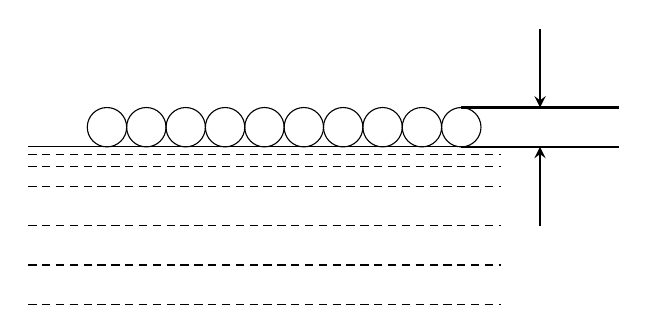
\begin{tikzpicture}[>=stealth]
\draw (0,0)--(6,0);

\foreach \x in {-.1, -.25, -.5, -1, -1.5, -2}
{ 
   \draw [densely dashed](0,\x)--(6,\x);
}

\foreach \y in {1,2,...,10}
{
   \draw (\y/2+.5,.25) circle [radius=.25];
}

\draw [thick] (5.5,0)--(7.5,0);
\draw [thick] (5.5,.5)--(7.5,.5);
\draw [->,thick](6.5,1.5)--(6.5,.5);
\draw [->,thick](6.5,-1)--(6.5,0);

\end{tikzpicture}

\caption{水面上的单分子油膜的示意图}
\end{figure}

    现在有了能放大上百万倍的离子显微镜,用它可以看到
钨针针尖上原子分布的图样,并且可以测出
钨原子间的距离大约是$2\times 10^{-10}$米,设想钨原子是一个挨着
一个排列的,那么,可以认为钨原子间的距离$2\times 10^{-10}$米就是
钨原子的直径.

    物理学中有各种不同的方法来测定分子的大小.用不同
方法测出的分子的大小并不完全相同,但是数量级是相符的.
测定的结果表明,一般分子直径的数量级都是$10^{-10}$米.例
如水分子的直径是$4.0\times 10^{-10}$米,氢分子的直径是$2.3\times 10^{-10}$
米.

    需要指出的是:把分子看作小球,是分子运动论中对分子
的简化模型;实际上,分子有它复杂的内部结构,并不真是小
球.因此,说分子的直径有多大,一般知道数量级已经可以
了,它提供了关于分子大小的一个数量观念,使我们了解分子
是多么微小.

    \subsection{阿伏伽德罗常数}

我们在化学课中学过,1摩尔\footnote{摩尔简称摩,国际符号是mol}
的任
何物质,其中含有的粒子数相同,都等于12克碳-12中含有
的原子数,这个数叫做\textbf{阿伏伽德罗常微}.

    知道分子的大小,可以粗略地算出阿伏伽德罗常数.例
如1摩的水,质量是$1.8\times 10^{-2}$千克,体积是$1.8\times 10^{-5}{\rm m}^3$.水
分子的直径是$4.0\times 10^{-10}{\rm m}$,体积大约是$3\times 10^{-29}{\rm m}^3$.设想
水分子是一个挨一个排列的,我们可以算出1摩的水中所含
的分子数:
\[N=\frac{1.8\times 10^{-5}{\rm m^3/mol}}{3\times 10^{-20}{\rm m^3}}=6\times 10^{23}{\rm mol}^{-1} \]

    早期测定阿伏伽德罗常数的一种方法,就是利用油膜法
测出分子直径,得出这个常数的.这种测定方法比较粗略,但
得出的数量级是正确的.

    我们看到,阿伏伽德罗常数是一个十分巨大的数字.为
了说明这个数字有多么大,我们设想有一个极小的动物来喝
水,它每秒钟喝进100亿个分子,要二百万年才能把1摩的水
喝完.

    反过来,知道了阿伏伽德罗常数,对液体和固体很容易估
算分子的大小.知道液体和固体的摩尔体积,设想其中的分
子是一个挨一个排列的,利用阿伏伽德罗常数就可以算出一
个分子所占的体积,从而估算出它的直径.

    知道了阿伏伽德罗常数,还可以算出分子的质量.水的
摩尔质量是$1.8\times 10^{-2}{\rm kg/mol}$,1摩的水中含有$6\times 10^{23}$个
分子,所以一个水分子的质量是
\[m_{\rm H_2 O}=\frac{1.8\times 10^{-2}{\rm kg/mol}}{6\times 10^{23}{\rm mol}^{-1}}=3\times 10^{-26}{\rm kg} \]
可见水分子的质量是很小的.除了包含几千个原子的有机物
大分子而外,一般分子的质量也是这个数量级.

    反过来,知道分子的质量,也可以算出阿伏伽德罗常数,
物理中有办法测出分子的质量,例如精确测得一个碳原子的
质量是$1.995\times 10^{-36}$千克,由此不难得出阿伏伽德罗常数.

    阿伏伽德罗常数是微观世界的一个重要常数,用分子运
动论定量地研究热现象经常要用到它,它是联系微观世界和
宏观世界的桥梁.从上面所讲的我们可以看出,阿伏伽德罗
常数把摩尔质量或摩尔体积这种宏观物理量跟分子质量或分
子大小这种微观物理量联系起来了.

    正因为阿伏伽德罗常数这样重要,所以物理学家们想出
各种办法来测定它,一百多年以来不断努力来更精确地测定
它,后面我们讲到电学的时候,就要提到一种测定阿伏伽德
罗常数的方法.现在测得的阿伏伽德罗常数的精确值是
\[N=6.022045\times 10^{23}{\rm mol^{-1}} \]
通常可取作
\[N=6.02\times 10^{23}{\rm mol^{-1}} \]

\section*{阅读材料:离子显微镜}
    课文中提到,用离子显微镜可以测出钨原子的直径.现
在简单介绍一下离子显微镜的构造和原理.

    离子显微镜由半径约为10厘米的球形玻璃容器和一根
钨针组成,钨针的针尖放在容器的中心(图1.2).针尖的表面
可以看作是半径非常小的球面,近代金属加工技术可以做到
使这个半径约为$5\times 10^{-6}$厘米.在球形容器的内表面涂上一
薄层导电物质,象电视荧光屏那样,在快速粒子打击下可以发
光.在导电层和针尖之何加上高电压,使导电层带负电,针尖
带正电.

\begin{figure}
\centering
\includegraphics[scale=.8]{fig/1-2.png}
\caption{离子显微镜的构造原理
}
\end{figure}


    在球形容器中充满低压的氦气.当无规则运动的氦原子
与针尖上的钨原子碰撞时,由子氦原子失去电子成为正离子,
氦离子在电力作用下就离开针尖,以很大速度沿着球半径运
动,打到球形容器的内表面上使之发光.这样,就出现了钨针
针尖上原子分布的图样(图1.3).

\begin{figure}
\centering
\includegraphics[scale=.8]{fig/1-3.png}
\caption{计算离子显微镜的
放大倍数,图中的
$a$和$b$表示钨针针
尖上的两个钨原子;
$A$和$B$分别表示它
们在球形容器内表
面上的像.$R$是球
形容器的半径,$r$表
示针尖的半径.
}
\end{figure}

    图1.3中弧长$ab$表示相邻两个钨原子间的距离,弧长$AB$
表示它们在球形容器内表面上的像之间的距离.因为$AB=R\alpha$, $ab=r\alpha$,
所以放大倍数
\[K=\frac{AB}{ab}=\frac{R}{r}=\frac{10{\rm cm}}{5\times 10^{-6}{\rm cm}}=2\times 10^5 \]
即放大二百万倍.已知放大倍数,测出弧长$AB$,就可以
求出原子间的距离$ab$.设想钨原子是一个挨一个排列的,可
以认为距离$ab$等于钨原子的直径.测定结果表明,钨原子的
直径是$2\times 10^{-10}$米.


\subsection*{练习一}
\begin{enumerate}
\item  一般分子的直径,以厘米作单位时数量级是多大?
\item  把体积为1$\rm mm^3$的石油滴在水面上,石油在水面上
形成面积为3$\rm m^2$的单分子油膜.试估算石油分子的直径.
\item  设想把分子一个挨一个地排起米,要多少个分子才
能排满1米的长度?
\item  1$\rm cm^3$水中含有多少个水分子?10克氧中含有多少
个氧分子?
\item  一个氧分子、一个氮分子的质量各是多少千克?
\item  已经测得一个碳原子的质量是$1.995\times 10^{-26}$千克,
求阿伏伽德罗常数.
\item  已知金刚石的密度是$3500{\rm kg/m^3}$,有一小块金刚
石,体积是$5.7\times 10^{-8}{\rm m^3}$.这小块金刚石中含有多少个碳原
子?设想金刚石中碳原子是紧密地堆在一起的,估算碳原子的
直径.

\end{enumerate}







\section{布朗运动}
物体里的分子永不停息地做无规则运动,这个结论也是在实验事实的基础上得到的.我们在初中学过的扩散现象表明分子在不停地运动.现在我们再讲一种现象,它可以更明
显地证实分子的无规则运动,这种现象叫做布朗运动.

1827年英国植物学家布朗用显微镜观察悬浮在水中的花粉,发现花粉颗粒不停地做无规则运动,后来把颗粒的这种无规则运动叫做布朗运动.不只是花粉,悬浮在液体中的微粒,都做布朗运动,把少量墨汁用水稀释,取一滴这样的液体放在显微镜下来观察(图1.4),就可以看到碳粒做无规则
的布朗运动,图1.5是做布朗运动的三个微粒的运动路线,从图中可以看出,布朗运动是毫无规则的.这个图只画出了
每隔30秒观察到的微粒的位置,并用直线依次把这些位置连接了起来.实际上,即使在这短短的30秒内,微粒的运动也是极不规则的.

\begin{figure}[htp]
\centering
\includegraphics[scale=.8, angle=1]{fig/1-4.png}
\caption{观察布朗运动的装置的示意图(左),
右图是显微镜下看到的微粒
}
\end{figure}

\begin{figure}[htp]
\centering
\includegraphics[scale=1.2]{fig/1-5.pdf}
\caption{做布朗运动的微粒的运动路线
}
\end{figure}


布朗运动是怎样产生的呢?起初,人们认为是由外界影响如震动、液体的对流等引起的.但是实验表明,在尽量排除外界影响的情况下布朗运动仍然存在.只要微粒足够小,在任何液体中都可以观察到布朗运动.布朗运动决不会停止.我们可以连续观察许多天甚至几个月,也看不到这种运动会停下来.
可见布朗运动的原因不在外界,而在液体内部.
\begin{figure}[htp]
\centering
\includegraphics[scale=1.2]{fig/1-6.pdf}
\caption{
}
\end{figure}

甚至在显微镜下看起来是连成一片的液体,实际上也是由许许多多做不规则运动的分子组成的,悬浮在液体中的微粒不断地受到液体分子的撞击,图1.6描绘了一个微粒受
到液体分子撞击的情景.当微粒足够小时,它受到的来自各个方向的液体分子的撞击作用是不平衡的.在某一瞬间,微粒在某个方向受到的撞击作用强,它就沿着这个方向运动,在下一瞬间,微粒在另一方向受到的撞击作用强,它又向着另一方向运动,这样,就引起了微粒的无规则的布朗运动.悬浮在液体中的颗粒越小,在某一瞬间跟它相撞的分子数越少,撞击作用的不平衡性就表现得越明显,因而布朗运动越明显.悬浮在液体中的颗粒越大,在某一瞬间跟它相撞的分子数越多,撞击作用的不平衡性就表现得越不明显,以至可以认为撞击
作用相互平衡,因而布朗运动越不明显以至观察不到.

可见,液体分子永不停息的无规则运动是产生布朗运动的原因.分子的运动我们是看不见的,做布朗运动的微粒是由成千上万个分子组成的,微粒的布朗运动并不是分子的运动,但是微粒的布朗运动的无规则性,却反映了液体内部分子运动的无规则性.

实验表明,布朗运动随着温度的升高而愈加微烈.在扩散现象中,也是温度越高,扩散进行得越快,这表示分子的无规则运动跟温度有关系,温度越高,分子的无规则运动越激烈.正因为分子的无规则运动跟温度有关系,所以通常把分子的这种运动叫做热运动.


\subsection*{练习二}
\begin{enumerate}
\item 有人说布朗运动就是分子的运动,这种说法对吗?为什么?
\item 为什么悬浮在液体中的颗粒越小,它的布朗运动越明显?为什么悬浮在液体中的颗粒越大,它的布朗运动越不明显以至观察不到?
\item 为什么说布朗运动的无规则性反映了液体内部分子运动的无规则性?设想液体内部分子的运动是有规则的,比如在任何时刻所有分子都向着某个方向运动,还能不能产生布朗运动?
\item  图1.5中所示的不同小颗粒的布朗运动的情况并不相同,人们由此考虑到布朗运动不可能是由外界影响引起的.为什么?找几位同学一起讨论一下,并说明你的理由.
\end{enumerate}

\section{分子间的相互作用力}
布朗运动和扩散现象不但说明分子不停地做无规则运动,同时也说明分子间是有空隙的,否则分子便不能运动了.气体容易被压缩,水和酒精混合后的体积小于两者原来体积之和,说明气体分子之间、液体分子之间都有空隙.有人曾用两万标准大气压的压强压缩钢筒中的油,发现油可以透过筒壁逸出,说明钢的分子之间也有空隙.前面讲述分子的大小时,认为面体分子和液体分子是一个挨一个排列的,那只是为估算分子直径的数量级而作的设想.

分子间虽然有空隙,大量分子却能聚集在一起形成固体或液体,说明分子之间存在着引力.用力拉伸物体,物体内要产生反抗拉伸的弹力,就是因为分子间存在着引力的缘故.把两块纯净的铅压紧,由于分子间的引力,两块铅就合在一起,甚至下面吊一个重物也不能把它们拉开.把两块光学玻璃的表面磨得很光滑又相吻合,把表面处理干净,施加一定的压力就可以把它们粘合在一起,这也是利用了分子间的引力.

分子间有引力,而分子间又有空隙,没有紧紧吸在一起,这说明分子间还存在着斥力.面体和液体很难被压缩,即使气体,压缩到一定程度后再继续压缩也很困难,就是因为分子间存在着斥力的缘故,用力压缩物体,物体内要产生反抗压缩的弹力,就是分子间的斥力的表现.

研究表明,分子间同时存在着引力和斥力,它们的大小都跟分子间的距离有关.图1.7甲中的两条虚线分别表示两个
分子间的引力和斥力随距离变化的情形,实线表示引力和斥力的合力即实际表现出来的分子间的作用力随距离变化的情形.我们看到,引力和斥力都随着距离的增大而减小,当两分子间的距离等于$r_0$时,分子间的引力和斥力相互平衡,分子间的作用力为零.$r_0$的数量级约为$10^{-10}$米,相当于距离为$r_0$的位置叫做平衡位置.当分子间的距离小于$r_0$时,引力和斥力虽然都随着距离的减小而增大,但是斥力增大得更快,因而分子间的作用力表现为斥力.当分子间的距离大于$r_0$时,引力和斥力虽然都随着距离的增大而减小,但是斥力
减小得更快,因而分子间的作用力表现为引力,它随着距离的增大迅速减小,当分子间的距离的数量级大于$10^{-9}$米时,已
经变得十分微弱,可以忽略不计了.
\begin{figure}[htp]\centering
	\includegraphics[scale=.8]{fig/1-7.pdf}
	\caption{分子间的作用力跟距离的关系.图甲中斥
力用正值来表示,引力用负值来表示.合力
$F$为二者的代数和.合力为正值时,表示合
力为斥力;合力为负值时,表示合力为引力.
}
\end{figure}

我们知道,分子是由原子组成的,原子内部有带正电的原子核和带负电的电子.分子间这样复杂的作用力就是由这些带电粒子的相互作用引起的.

上面我们讲了分子运动论的基本内容,分子不停地做无规则运动,它们之间又存在相互作用力,分子力的作用使分子聚集在一起,分子的无规则运动将使它们分散开来,由大量分子组成的物体可以处于气、液、固三种不同的物质状态,正是由这两种相反的因素决定的,在面体中,分子力的作用比较强大,绝大多数分子被束缚在平衡位置附近做微小的振动.温度升高,分子的无规则运动加剧,加剧到一定限度,分子力的作用已经不能把分子束缚在固定的平衡位置附近,但分子还不能分散远离,于是物体表现为液体状态.温度再升高,分子的无规则运动更加剧,到一定限度,分子分散远离,分子力的作用很微弱,分子可以到处移动,物体就表现为气体状态.

\subsection*{练习三}
\begin{enumerate}
	\item 什么事例说明分子间有引力?什么事例说明分子间有斥力?
	\item 当分子间的距离大于$r_0$时,随着距离的增大,引力和斥力哪个减小得快?当分子间的距离小于$r_0$时,随着距离的减小,引力和斥力哪个增加得快?
	\item 物体为什么能够被压缩,但又不能无限地被压缩?
\item	从图1.7看出,当分子中心间的距离小于$r_0$时,分
子间的作用力表现为斥力,它随着距离的减小而很快地增大.分子间作用力的这一特点,可以借助于下述模型想象出来.设想分子为弹性钢球,当两个钢球相撞时,它们都发生微小的形变,因而在它们之间产生相互推斥的弹力,如同分子间的作用力表现为斥力一样.钢球发生微小形变就可以产生很大的弹力,所以这个弹力随着钢球中心间距离的减小而很快地增大.利用这一模型可以粗略地估计出分子直径的数量级为$10^{-10}$米.这是怎样估计的?

\end{enumerate}

\section*{复习题}
\begin{enumerate}
\item 分子运动论的基本内容是什么?
\item 就你所知道的,测定分子的大小和阿伏伽德罗常数有什么方法?
\item 什么叫布朗运动?布朗运动是怎样产生的?为什么把大量分子的无规则运动叫做热运动?
\item 仔细研究图1.7,说明分子间作用力的特点.
\end{enumerate}















